\documentclass[class=article, crop=false]{standalone}
\usepackage[utf8]{inputenc}
\usepackage{graphicx}
\renewcommand{\baselinestretch}{1.5} 
\usepackage{wrapfig}
\usepackage{subcaption}
\usepackage{caption}
\usepackage{float}
\usepackage{xcolor}
\usepackage{amsmath}
\usepackage{blindtext}
\usepackage{import}
% \usepackage[backend=biber, style=numeric, citestyle=nature, doi=false, isbn=false, url=false, eprint=false]{biblatex} % Imports biblatex package, Comment out main doc
% \addbibresource{refs.bib} %Import the bibliography file, Comment out main doc

\begin{document} 
\label{section:Introduction}

Magnetic resonance imaging (MRI) or spectroscopy (MRS) scans look at the abundance of a particular nuclei \textit{in vivo}, the most common used as reference is the hydrogen nuclei ($^1$H) which consists of a negatively charged electron orbiting a positive charged proton. This is due to the fact that $^1$H is the most abundant nuclei in the human body with an adults bodyweight being made up of ~60\% water (H$_2$O) and can be estimated based on someones age, sex, height and weight\cite{Watson1980TotalMeasurements}. This means that tissues that have a larger H$_2$O abundance will have a stronger MR signal. Whilst in general this is useful as it can generate images or spectra with a high signal-to-noise ratio (SNR), it can be difficult to measure small differences in substances with a strong MR signal. In order to investigate, measure and quantify metabolism it is vitally important to be able to measure small differences in the products that are created due to metabolism (metabolites). Therefore, often other reference nuclei are often used to investigate metabolism, it is important to choose a nuclei that is magnetically favourable and is chemically bound to metabolites that are of interest. Carbon-13 ($^{13}$C)\cite{Grist2019QuantifyingImaging,Brender2019DynamicHyperpolarization} and Phosphorous-31 ($^{31}$P)\cite{Gordon1980LocalizationResonance} are often used in research to quantify metabolite concentrations \textit{in vivo}, due to their lower abundance in the human body (compared to $^1$H), whilst still being magnetically favourable for MRS studies. Their abundances are too low for direct MRI measurements, and the ability to separate different metabolites in each spectrum is important. Recently deuterium ($^2$H) has been shown to be a nuclei of interest when investigating metabolism in humans \textit{in vivo}\cite{Lu2017QuantitativeSpectroscopy,DeFeyter2018DeuteriumVivo}, and since then the field has grown at a very fast rate thanks to its capabilities in viewing brain tumours\cite{DeFeyter2018DeuteriumVivo} along with its relatively simple implementation.

\begin{figure}
    \centering
    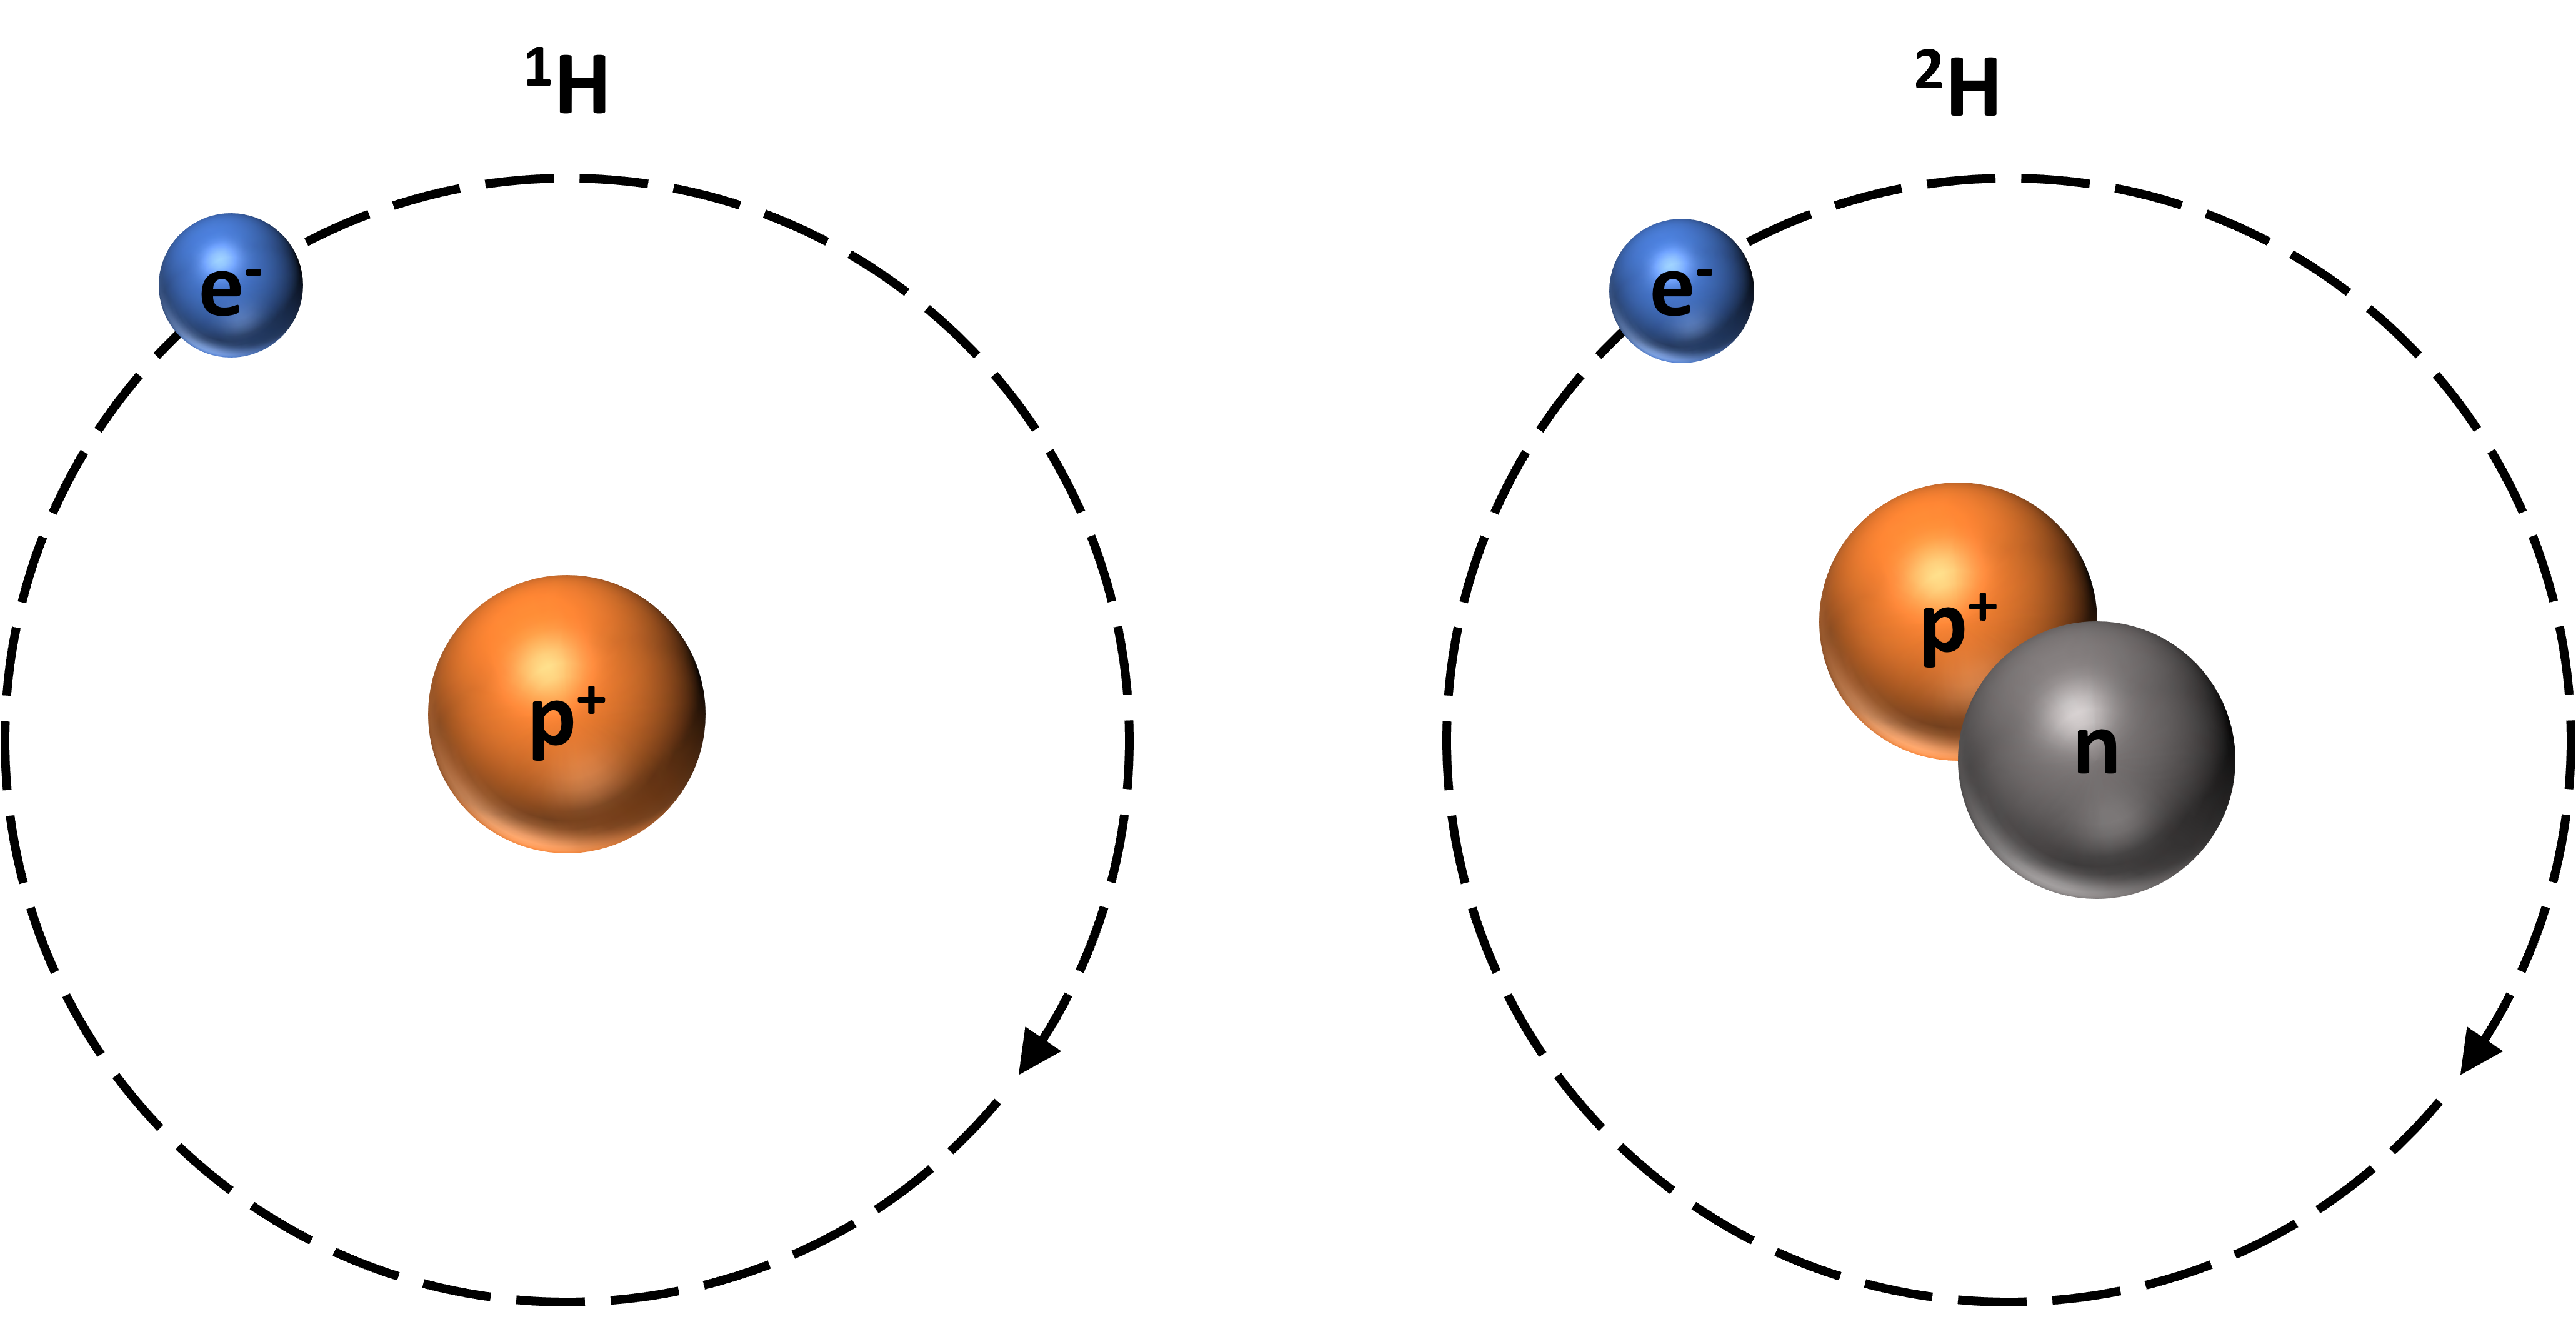
\includegraphics[width=0.9\textwidth]{Figures/Intro/1H2H.png}
    \caption{Atomic diagram of hydrogen ($^1$H, left) and deuterium atoms ($^2$H, right).}
    \label{fig:intro:1H2H}
\end{figure}

\section{Metabolism}

Metabolism is a key aspect of many life-altering diseases including cancer and neurodegenerative diseases, such as Alzheimer's disease (AD), Parkinson's Disease (PD) and Multiple Sclerosis (MS)\cite{Gialleonardo2016TheImaging}. AD has a European age-standardized prevalence of 4.4\% among people aged over 65\cite{Qiu2009EpidemiologyIntervention}. One of the most prevalent and fatal metabolic diseases is cancer, in 2017 there were ~375,000 new cancer cases in the UK\cite{CancerUK}, with ~3\% of them being attributed to Brain, other CNS and intracranial tumours\cite{BrainUK}. With the mortality rate of these tumours having remained stable for the last decade\cite{BrainUK}. This shows the importance of researching metabolism \textit{in vivo}, and more specifically brain tumours.

\begin{figure}
    \centering
    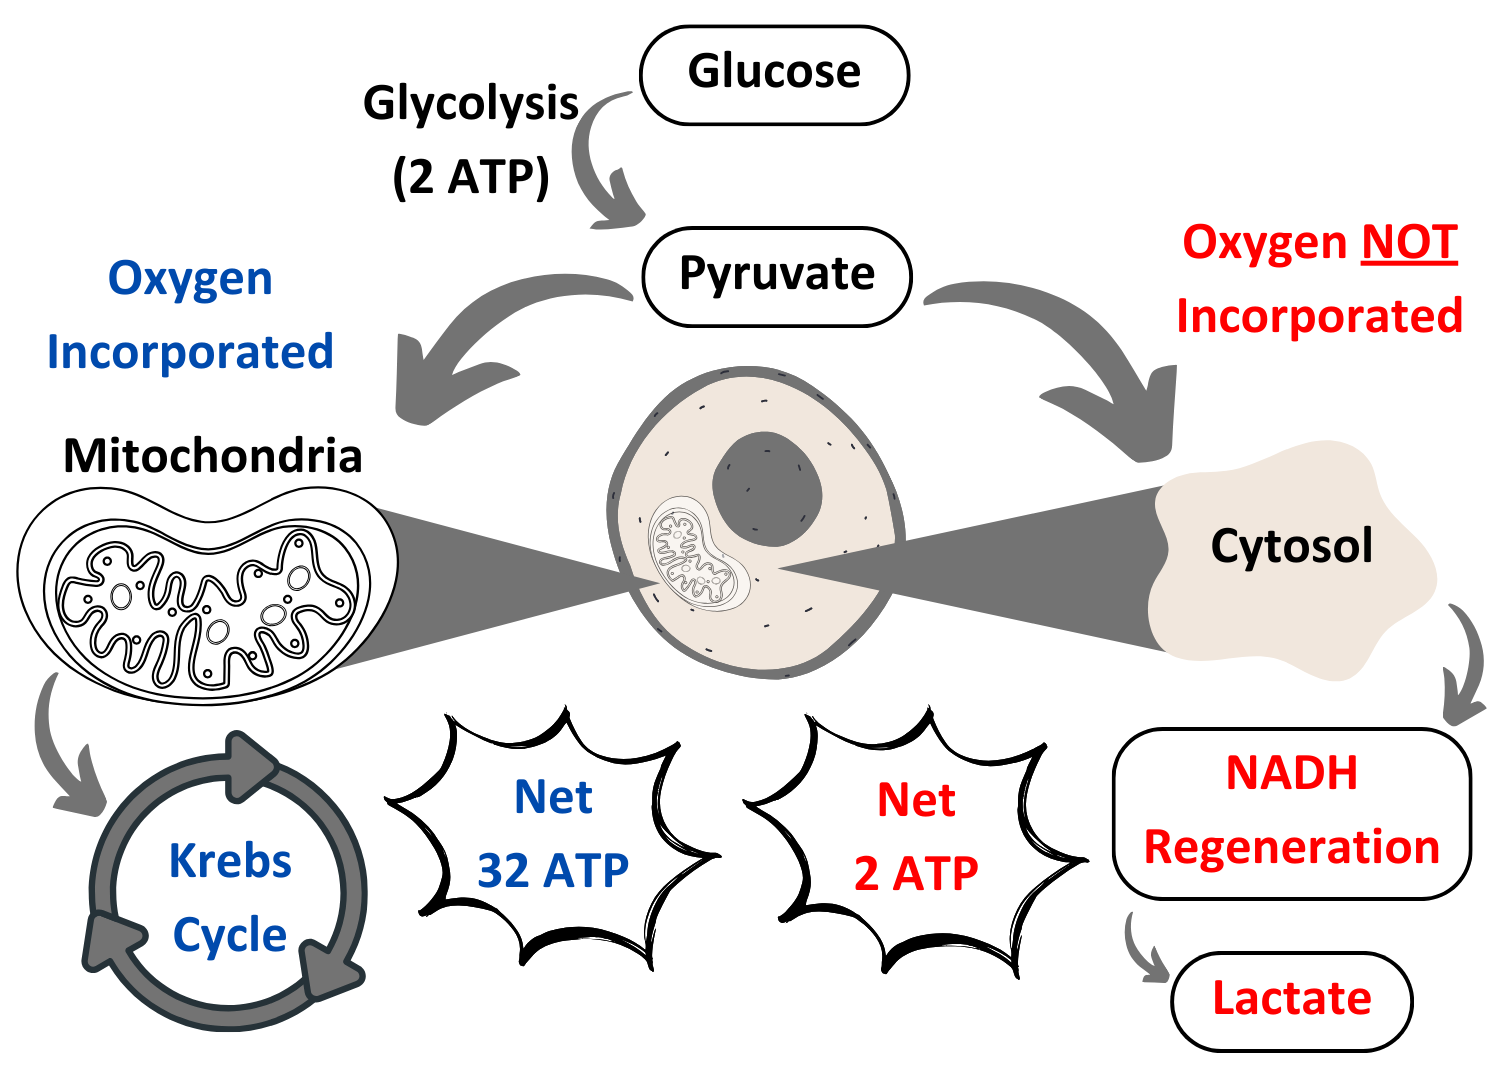
\includegraphics[width=0.75\textwidth]{Figures/Intro/Metabolism.png}
    \caption{Flow Chart demonstrating how glucose is metabolised into ATP with (aerobic, blue) and without (anaerobic, red) oxygen being present. Healthy cells favour aerobic respiration whilst cancerous cells prefer anaerobic respiration.}
    \label{fig:intro:Metabolism}
\end{figure}

Cancers and tumours are often considered as a metabolic diseases because as part of their growth and function they affect and impair normal metabolism. In cells the nucleic acid adenosine triphosphate (ATP) is how cells store energy through the breakdown of ATP. In mammalian cells pyruvate is generated from glucose via glycolysis and produces two moles of ATP per each mole of glucose. In healthy cells there are then two options for metabolism depending on the supply of oxygen to the cell, if oxygen is in readily supply a process called oxidative phosphorylation (oxphos) takes place. Oxphos is where pyruvate enters the mitochondria and the citric acid (also known as the tricarboxylic acid (TCA) or Krebs) cycle where thirty-two more ATP are produced. This complete process is often referred to as aerobic respiration. The other option, when oxygen is not in readily supply, is when pyruvate is converted into lactate in the cytosol of the cell through NADH regeneration. The complete process for the creation of lactate is known as lactic acid fermentation. Aerobic respiration is much more efficient in its energy production producing ~sixteen times more ATP per mole of glucose compared to lactic acid fermentation\cite{Romero-Garcia2011TumorView}. Only the seven hydrogens that aren't present in hydroxyl groups in glucose are able to be replaced with $^2$H atoms. During Oxphos glutamate and glutamine are produced (combination of the two is referred to as glx) and of these seven hydrogen atoms only three are found in glutamine/glutamate. During lactic fermentation only three of the hydrogen atoms are found in lactate. These hydrogen's come from the C1, C6 and C6' positions in the glucose molecule. The rest of the labels (C2, C3, C4 and C5) are lost in the production of the water during lactic acid fermentation and aerobic respiration. Otto Warburg observed in the 20$^{th}$ century that tumours had a higher rate of glucose uptake\cite{WarburgBerlin-Dahlem1925TheCells,Warburg1956OnCells}. There were originally quite a few theories involving that cancerous cells had impaired the mitochondria. It is now thought that the reason behind this is that cancerous cells are able to metabolise by either Oxphos or by fermentation regardless of how much oxygen is present to the cell. Lactic fermentation is favoured to Oxphos even though it is less energy/ATP efficient which therefore leads to an increase in lactate and a decrease in glx present\cite{Romero-Garcia2011TumorView}.

\begin{figure}[ht]
    \centering
    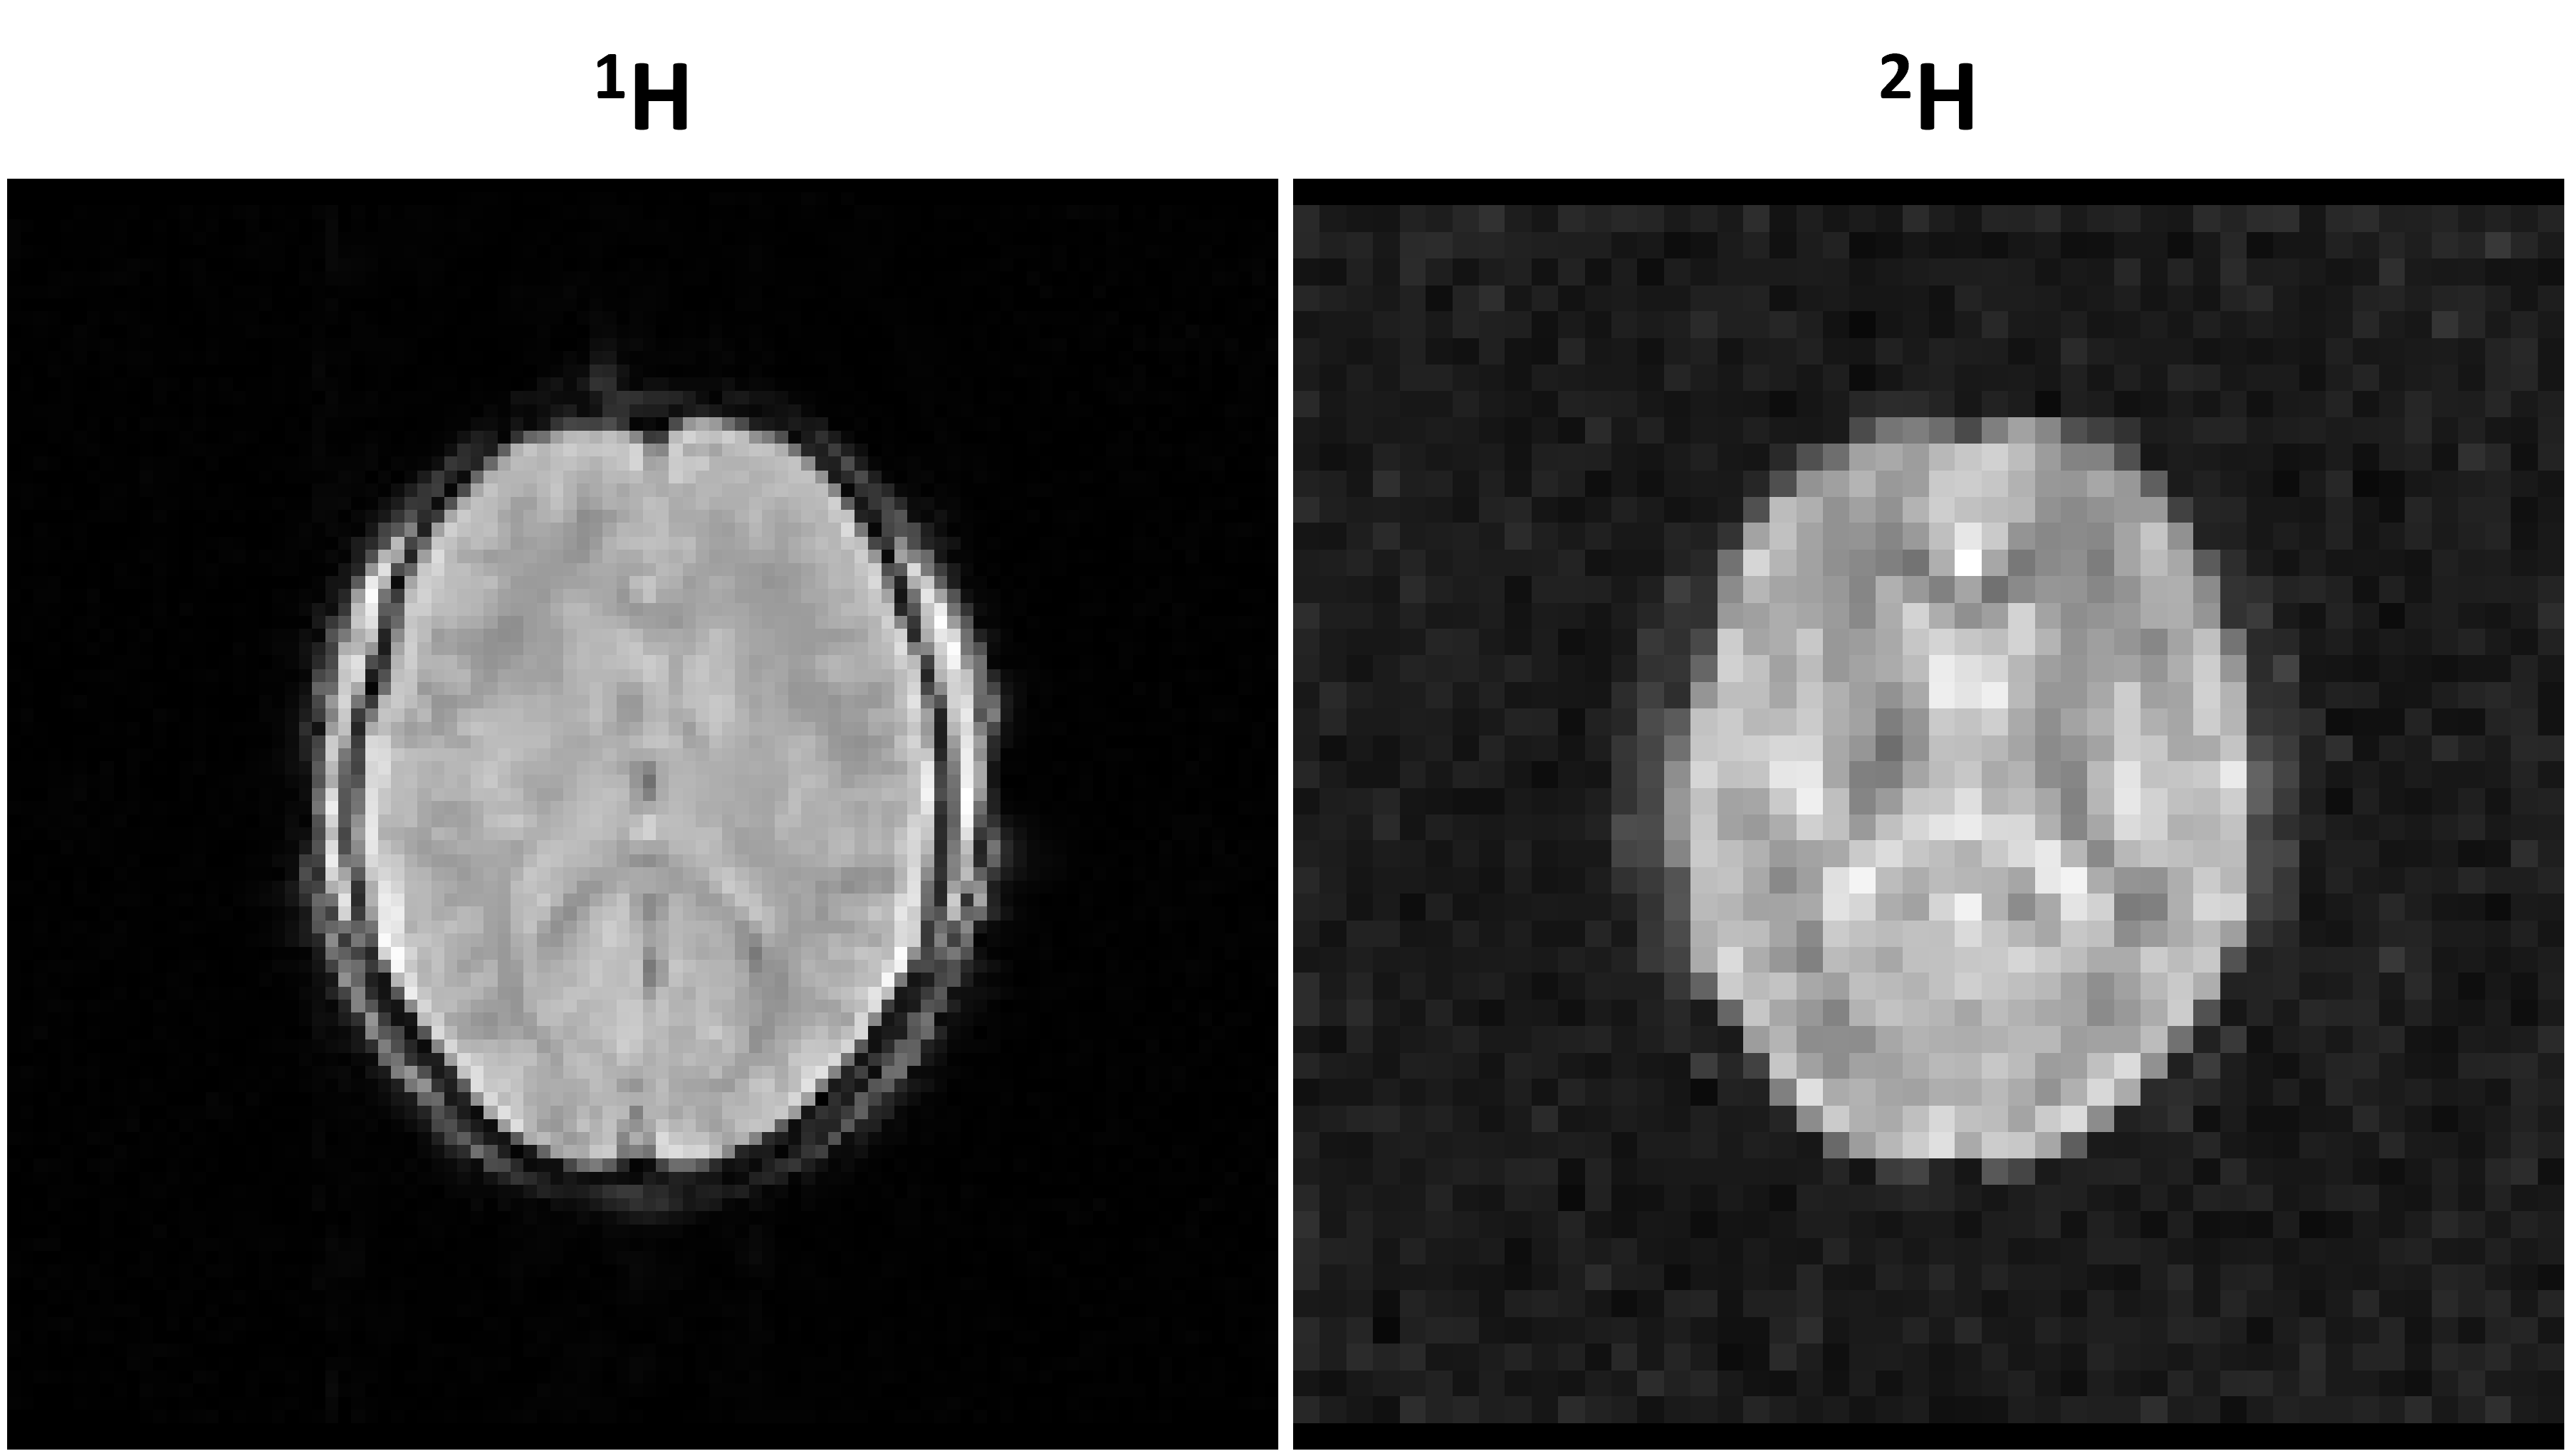
\includegraphics[width=0.9\textwidth]{Figures/Intro/1H2H_Brain.png}
    \caption{Scan images of the brain acquired at different nuclei Larmor Frequencies, for multi-echo gradient-echo (MEGE) in the same scan session for the same participant. Left is a $^1$H image with 3x3x2.5 mm$^3$ voxels acquired in 232 s. Right is a $^2$H image obtained with 6x6x10 mm$^3$ voxels with a scan duration of 354 s. It is important to note that the participant's $^2$H level is 100x natural abundance as they have consumed heavy water (D$_2$O) as part of a study.}
    \label{fig:intro:1H2H_Brain}
\end{figure}

Currently the most reliable way to accurately diagnose and monitor most cancers and metabolic diseases, in a non-invasive way, is by using positron emission tomography (PET) \cite{Almuhaideb201118F-FDGOncology}. Unfortunately this technique involves the use of a radioisotope inside the body which can put patients at further health risks, whilst a technique that revolved around MR would be both non-invasive and non-radioactive. Cancerous cells have a much higher glucose uptake during metabolism than normal cells. This is the basis behind PET imaging of cancer using $^{18}$F-labellled fluorodeoxyglucose (FDG), as the increased concentration of glucose of a specific tissue gives an indication of any cancerous tumours present. FDG PET works by attaching a positron emitting atom to a metabolite, such as glucose, once inserted into the body it travels to the tissues where glucose is needed most. The emitted positrons annihilate with electrons, creating two photons, which are then detected giving information on the location of the glucose and therefore information as to where cancer is present. Another problem with FDG PET is that because it only detects the presence of glucose it doesn't provide information on any downstream metabolites such as lactate. Since the brain is constantly metabolically active it can often be difficult to distinguish increases in metabolism compared to baseline, which is why it is important to choose a tracer with a low abundance. These metabolite signal/concentration maps are often displayed over high resolution anatomical images to provide accurate spatial distributions.

\begin{figure}
    \centering
    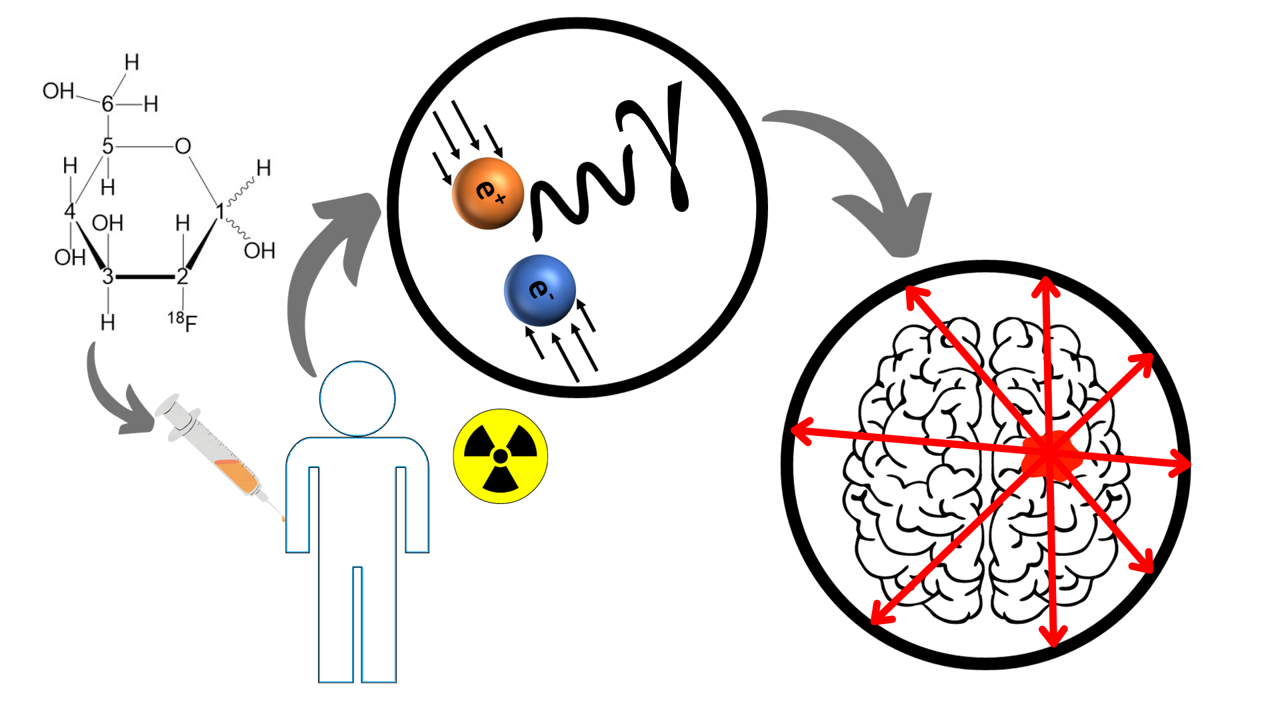
\includegraphics[width=1\textwidth]{Figures/Intro/PET_Scan.png}
    \caption{Diagram showing how positron emission tomography (PET) scanning works at detecting tumours.}
    \label{fig:intro:PET}
\end{figure}

\section{History}

\subsection{Pre-1980}

The reasoning behind why it took so long for the use in $^2$H in health and metabolism to take off is one of unfortunate timing, and to truly appreciate the reasoning's behind this we have to take a look at the beginning. $^2$H was discovered in 1932\cite{Urey1932AConcentration} to account for the apparent mass difference for hydrogen when measured chemically and with a mass spectrograph. From then it didn't take long for the realisation that this stable isotope could be used to measure metabolism. Many papers were released theorising and showing this\cite{Schoenheimer1935DeuteriumMetabolism,Schoenheimer1935DeuteriumMetabolismb,Schoenheimer1938TheMetabolism} which involved deuterating naturally occurring compounds such as fatty acids, feeding them to animals and then analysing the amount of deuterium found in bodily fluids. Shortly after this the relaxation properties of $^2$H in nuclear magnetic resonance (NMR) were quantified in a solution of heavy water\cite{Bloembergen1948RelaxationAbsorption}. One possible explanation as to why it then took so long for this technique combined with NMR to become popular is due to the rising interest (at the time)\cite{DeFeyter2021DeuteriumFuture} in radioactive isotopes $^3$H\cite{Thompson1953StudiesRat} and $^{14}$C\cite{Turteltaub1990AcceleratorDNA.}. The health concerns of radioactive isotopes pushed a resurgence of $^2$H metabolism research in the 1980's.

\subsection{1980 to the 21\textsuperscript{st} Century}

% Graphs of fat lipid changes from paper or from our own NA work 

\begin{figure}
    \centering
    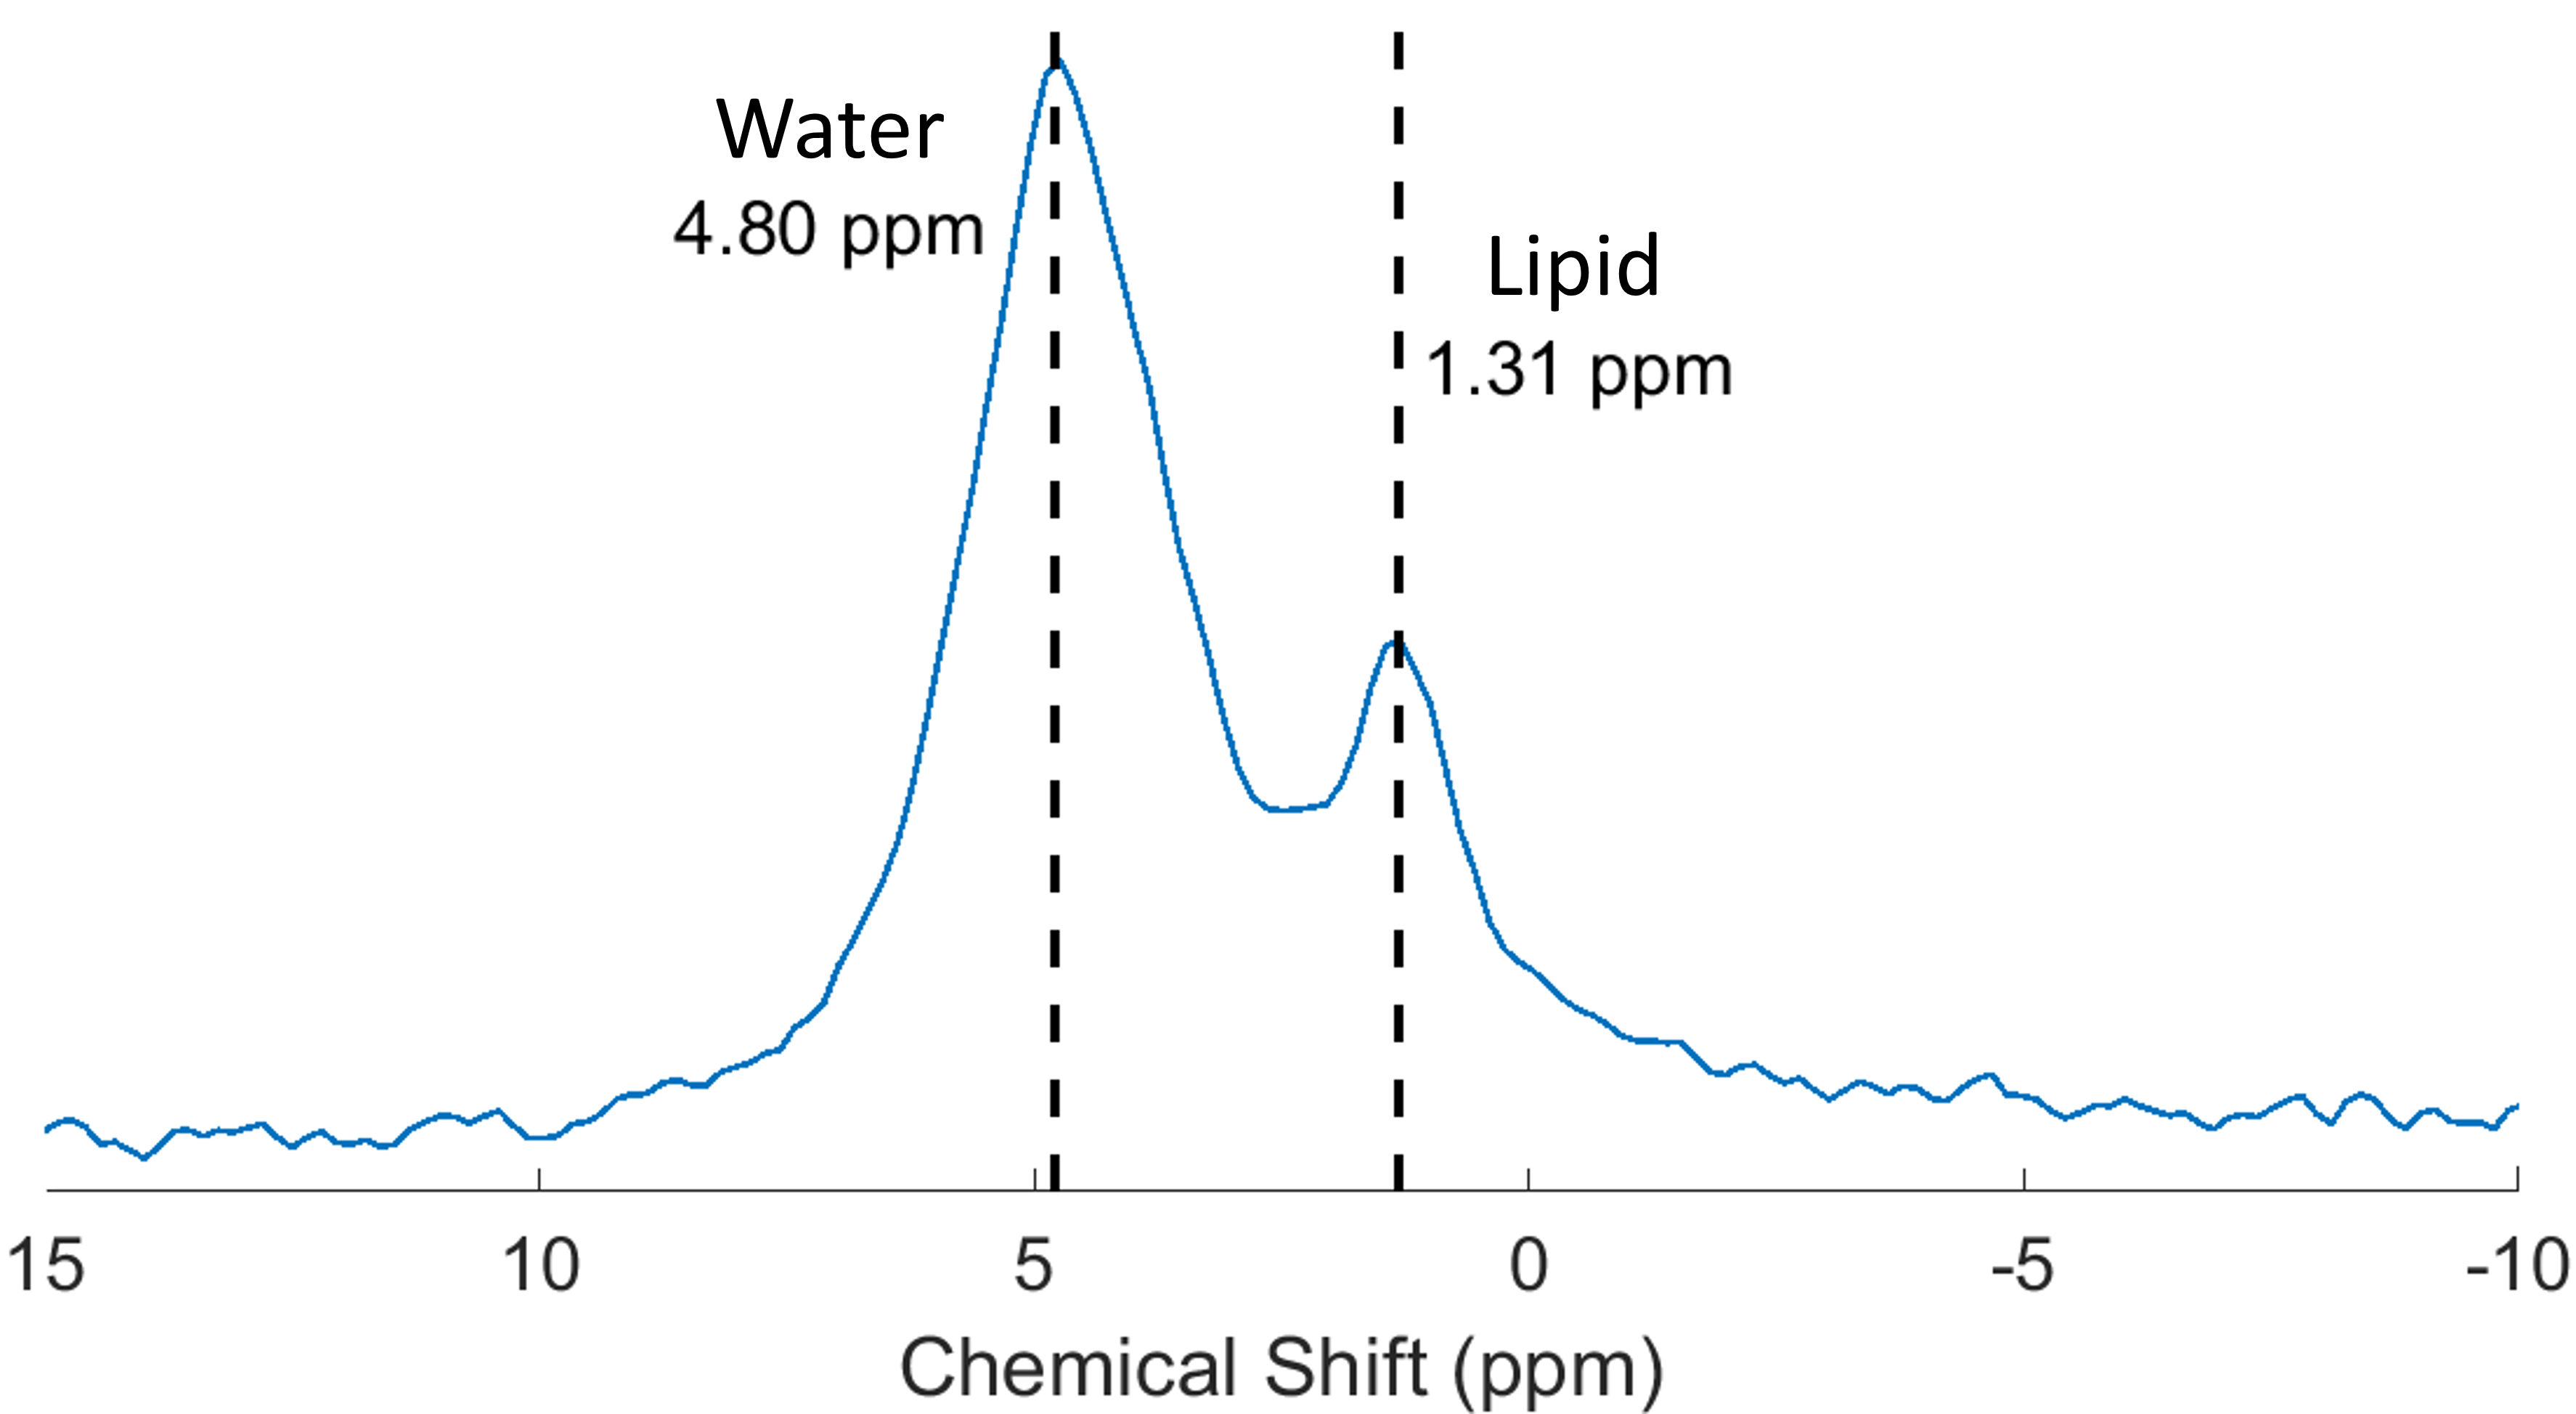
\includegraphics[width=0.8\textwidth]{Figures/Intro/NA_Spectra.png}
    \caption{Non-localised $^2$H spectra obtained from the calf \textit{in vivo} showing signals from water at a chemical shift of 4.8 ppm and fat/lipid signals at 1.3 ppm.}
    \label{fig:intro:NA}
\end{figure}

The first \textit{in vivo} NMR studies was performed in 1986\cite{Brereton1986PreliminarySpectroscopy} in mice models. Heavy water (D$_2$O) was ingested by mice to improve $^2$H abundance, where an increase in fat/lipid signal was noted. Shortly after this numerous studies were published that involved using heavy water as a tracer, looking at the brain\cite{Ewy1988DeuteriumSitu}, at blood flow and perfusion\cite{Ackerman1987DeuteriumTracer.} and looking at iron stores\cite{Irving1987InSpectroscopy}. Other deuterated compounds then started to be used such as choline\cite{Eng1990RenalStudy}, with the first instance of deuterated glucose being used being in 1986\cite{Barrow1986NMRMobilis}. This kicked off a trend of other studies using deuterated glucose to look at bacterial metabolism\cite{Aguayo1988HighMetabolism.} and liver gycogen synthesis\cite{Goodman1989UseSynthesis}. All the aforementioned studies involved animal models, the amount of studies that involved $^2$H began to slow down before a long haitus. One potential reason for this haitus is due to the success' of \textit{in vivo} $^1$H\cite{Harada1984IdentificationScience}, $^{13}$C\cite{Cohen1980UseLiver} and $^{31}$P\cite{Sappey-Marinier1992EffectSpectroscopy}. However, due to the technical difficulties of $^1$H and the expense of hyperpolarised (HP) $^{13}$C studies there is one final resurgence in $^2$H research and more specifically metabolism, hopefully ending this theme of unfortunate timing permanently. 

\subsection{The Last Seven Years}

\begin{figure}[H]
    \centering
    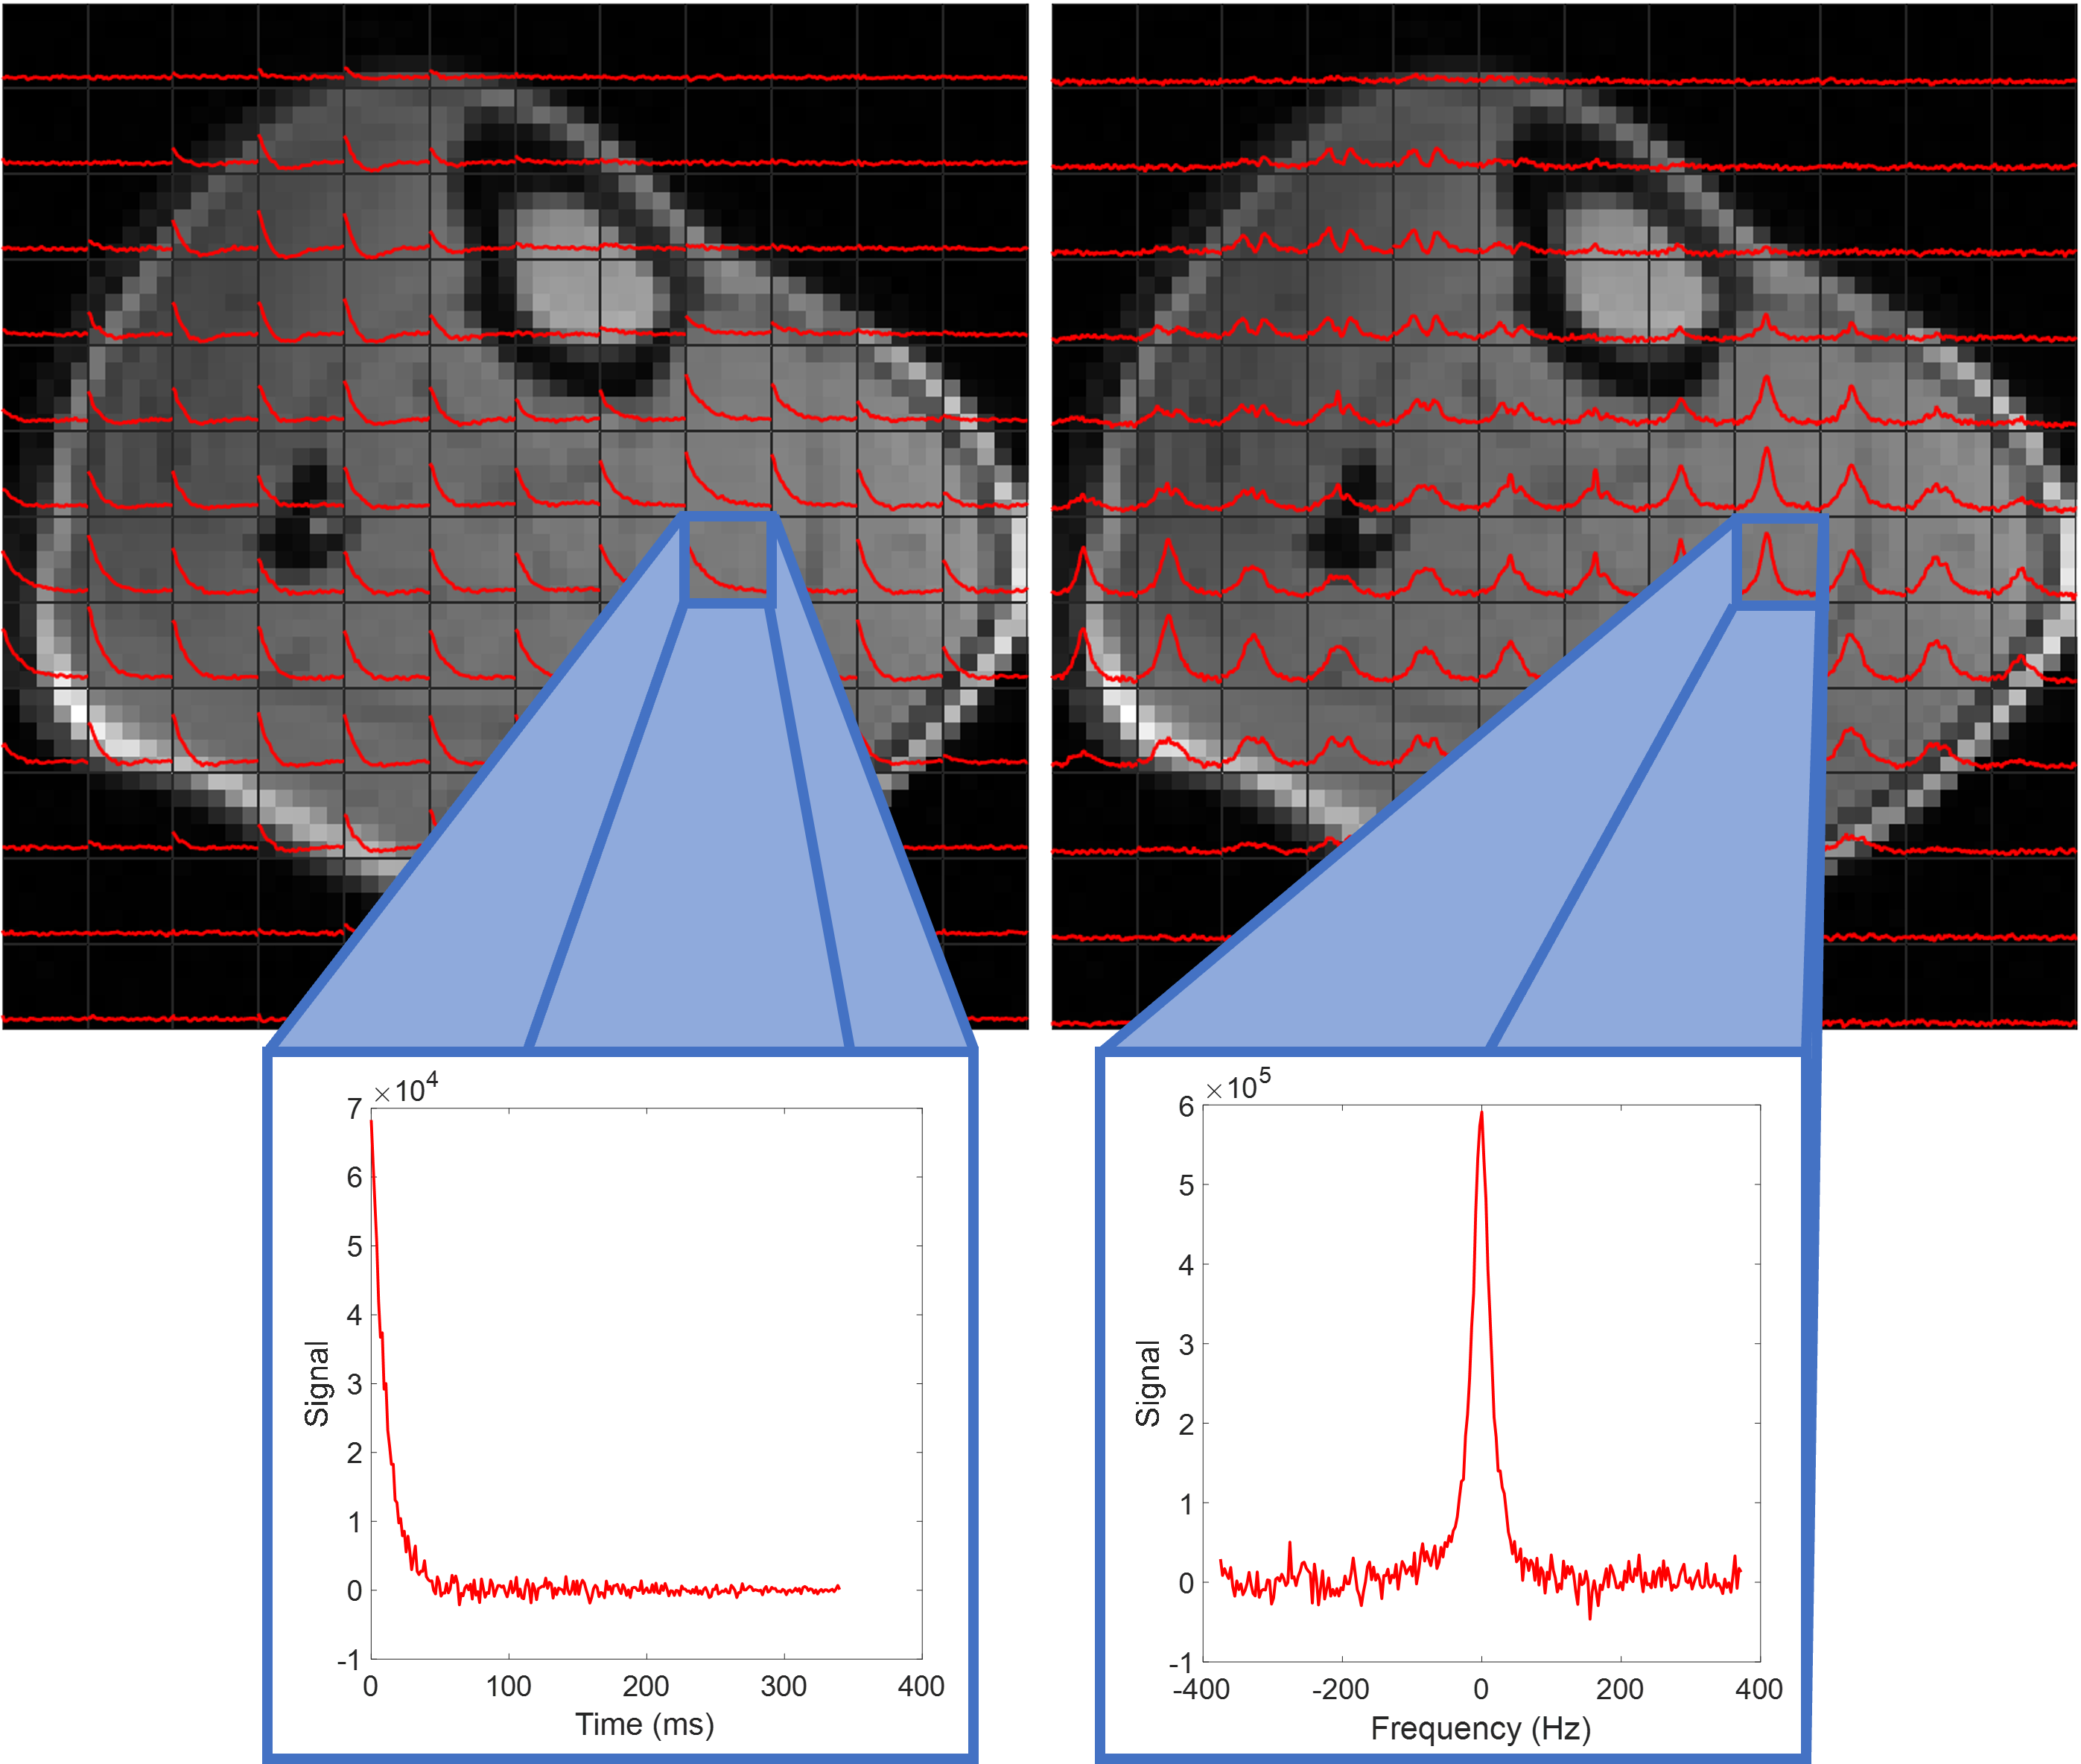
\includegraphics[width=0.8\textwidth]{Figures/Intro/CSI.png}
    \caption{Example natural abundance magnetic resonance spectroscopic imaging (MRSI) data overlayed onto an anatomical image of the Calf. The left shows voxels containing the localised FID data with one voxel blown up, the right shows the corresponding localised spectroscopic data (Fourier transform of the left) with data from one voxel blown up.}
    \label{fig:intro:CSI}
\end{figure}

It wasn't until 2017 when [6,6'-$^2$H$_2$] (also known as $^2$H$_2$-glucose or D$_2$-glucose) was used \textit{in vivo} in an animal model\cite{Lu2017QuantitativeSpectroscopy}. And it wasn't long until this technique was applied \textit{in vivo} in humans, where it was used to look at the contrast between normal and tumour tissue\cite{DeFeyter2018DeuteriumVivo}. This form of glucose is currently the most common used deuterated tracer that is currently used in research\cite{DeFeyter2018DeuteriumVivo,DeFeyter2021DeuteriumFuture,Ruhm2022Dynamic9.4T,Roig2022Deuterium7T,deGraaf2020OnImaging}. At natural abundance only one deuterated water (HDO) peak/signal is visible in a typical spectrum, because the noise level is larger than other signals present. After ingestion of D$_2$-glucose peaks from deuterated glucose (Glu), a combination of glutamine and glutamate (Glx) and lactate (Lac) become present. If enough localised spectra are acquired that span enough of the brain, by chemical shift imaging (CSI) or by another magnetic resonance spectroscopic imaging (MRSI) method, maps of each of these metabolites can be obtained. Maps of Glx and Lac are shown to give good healthy to diseased CNR in the brain, with maps of Glx divided by Lac giving the best CNR\cite{DeFeyter2018DeuteriumVivo,Straathof2021DeuteriumBrain}. Other deuterated compounds have been used to measure different metabolic pathways, such as [$^2$H$_3$]-acetate (D$_3$-acetate)\cite{DeFeyter2018DeuteriumVivo,Rich20201HVivo}, [6,6'-$^2$H$_2$]-fructose (D$_2$-fructose)\cite{Zhang202366-2H2Cancer}, as well as other forms of deuterated glucose being created such as [2,3,4,6,6'-$^2$H$_5$] (D$_5$-glucose)\cite{Zou2023AImaging} which is found to be cheaper than D$_2$-glucose. So as more studies are performed with patient cohorts, and as more deuterated compounds are investigated the field of metabolic imaging will continue to grow exponentially. 

% De Feyter images or CSI images

\section{Aims}

The wider aims of this thesis are to develop $^2$H MRI and MRSI scanning at the Sir Peter Mansfield Imaging Centre (SPMIC), University of Nottingham both at clinical high field 3T and at ultra-high field 7T. Work outlined in this thesis can theoretically be used to implement $^2$H at lower and higher field strengths. The more specific primary aim of this thesis is to set the ground-work for scanning patients with brain tumours using DMI at 7T, to improve the CNR between healthy and tumour tissue without the need for invasive and/or ionising radiation.

All the work that is therefore outlined in this thesis involves the use of MRI and MRSI techniques which covers calculating relaxation times for HDO in different healthy \textit{in vivo} brain tissues. Assessing the increase in $^2$H abundance as D$_2$O is ingested in in different healthy \textit{in vivo} brain tissues. Using different amounts of $^2$H labelling of glucose to assess \textit{in vivo} metabolism in the brain of healthy participants. Using the ingestion of D$_2$O to investigate is lipid turnover can be measured. Finally, using the ingestion of D$_2$O to assess the quadrupolar HDO splitting in anisotropic and isotropic tissues using regular MRI and MRSI as well as double quantum filtered MRI and MRSI.

\section{Description of Work}

Chapter two will cover the theory of the work that was undertaken in this thesis. This will include the theory behind MRI and MRSI and more specifically the difference between $^1$H and $^2$H, covering magnetisation, relaxation and pule sequences. It will also include the extra hardware adaptations that are needed for any $^2$H signal to be detected from amplifiers to RF coil building.

Chapter three summarises the work that involves the ingesting of D$_2$O. The reasoning behind why accurate relaxation times for different \textit{in vivo} tissues are important for quantification. A D$_2$O ingestion routine is outlined as well as a scanning routine undertaken that would allow the quantification of relaxation times using multi-echo gradient echo (MEGE) scans with different repetition times (TR), the same type of scans were then also used for some participants to track the $^2$H increase that occurs due to the ingestion of D$_2$O. It was shown that the $^2$H increase from MRI/MRS follows what is expected from blood sampling, and the relaxation times for different tissues are reported with statistical significance shown.

Chapter four gives an overview of some of the research that has been conducted so far in deuterium metabolic imaging (DMI) predicts the potential benefits of using D$_7$-glucose as opposed to D$_2$-glucose. The methodology used so healthy participants can ingest deuterated glucose is outlined as well as the scanning routine with parameters for CSI scanning. Increases in signal levels for all downstream metabolites resulting from the deuterated glucose are reported from the D$_7$-glucose which suggests better CNR between healthy and tumour tissue would be possible, despite the more complicated analysis.

Chapter five begins by demonstrating the importance of lipid turnover and the limitations of the present methodology involving biopsy, and suggests a new routine that uses MRI/MRS instead. A new routine of ingesting D$_2$O is given as well as regular scanning routine that is repeated once a fortnight. Increases in $^2$H lipid was seen in most the measurements with statistical significance, but new advances/improvements are needed to make this technique is clinically viable.

Chapter six gives the importance of investigating isotropic and anisotropic tissue ordering and how the quadrupolar interaction in $^2$H MRS provides this information. After participants have their $^2$H abundance increased by ingesting D$_2$O, MRSI and double quantum filtered (DQF) MRSI have been used to show the relationship between the anisotropy and quadrupolar interaction in the forearm and the calf.

Finally, chapter seven brings together all the work that has been conducted in this thesis, and gives direction on any future work that may be conducted.

% \printbibliography % Comment out main doc

\end{document}